\section{Co to jest raspberry pi?}
    
    \frame{\sectionpage}
    
    \begin{frame}{Raspberry Pi}
    
        \begin{block}{\centering Co to jest to Raspberry Pi?}
            Raspberry Pi - Urządzenie składa się z pojedynczego obwodu drukowanego i zostało wymyślone, by wspierać naukę podstaw informatyki. Jego premiera miała miejsce 29 lutego 2012 roku. Projekt rozwija Raspberry Pi Foundation.
        \end{block}
        \centering
        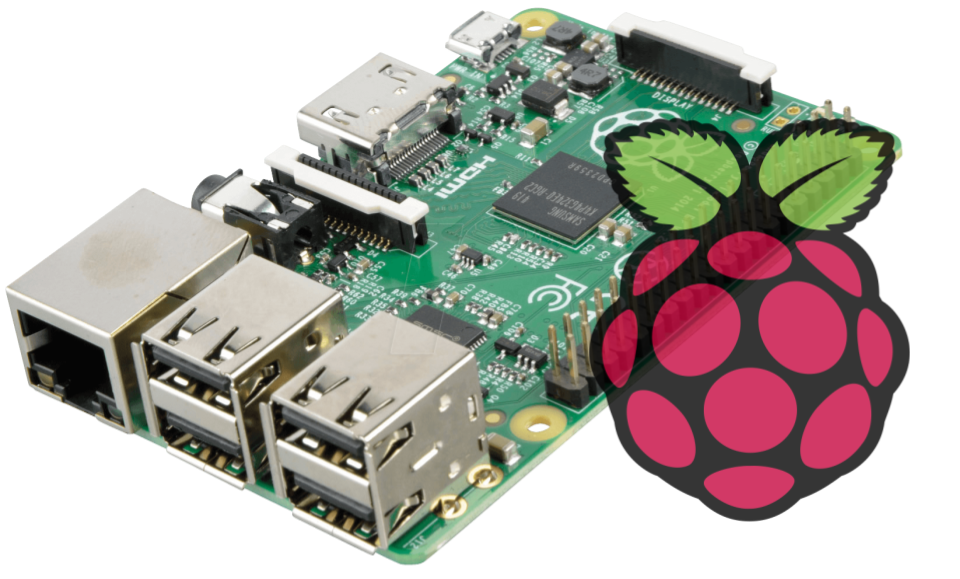
\includegraphics[height = 0.5 \textheight]{images/1pi.png}
    \end{frame}
    \begin{frame}{Modele Raspberry pi}

        \centering
        
\includegraphics[height = 0.5 \textheight]{images/2raspberry.png}
        \begin{table}[t]
            \begin{tabular}{|r|l|l|l|l|}
                \hline 
                    Model & 1 & 2 & 3 & 4\\
                \hline
                    Ram & 512MB & 1024MB & 1024MB & 4096 MB\\
                \hline
                    USB (ilość) & 4x 2.0 & 4x 2.0 & 4x 2.0 & 2x 2.0 i 2x 3.0\\
                \hline
                    Wi-FI & & & 802.11bgn & 802.11ac\\
                \hline
                    Bluetooth & & & 4.1, BLE & 5.0, BLE\\
                \hline
                \end{tabular}
            \end{table}
    \end{frame}